\section{Model Proposals}

In this section, we use the Box–Jenkins methodology to develop and assess SARIMA models for log-transformed and differenced time series data.
Then, we evaluated the residuals for white noise behaviour, checking for autocorrelation and verifying the statistical significance of the model coefficients.
This rigorous process ensures that the chosen model is statistically valid and suitable for forecasting.\\

To rigorously compare different modeling methodologies, we developed multiple candidate models based on the transformed and stationary series. Given the complexity and structure of the time series, specifically the presence of seasonality, a slight trend, and possibly varying variance, it is essential to explore alternative approaches.\\

The primary objective of this project is to evaluate the effectiveness of each model type in both the training and forecasting phases. To that end, we compare the model fit criteria and diagnostics in this section (Section 3), and evaluate predictive performance metrics in Section 4. This allows us to strike a balance between in-sample accuracy and out-of-sample generalization, while avoiding overfitting.

Since the models will later be used for forecasting, we previously split the dataset into training and test sets. All models are trained exclusively on the training set to prevent data leakage. 

\subsection{Box-Jenkins Methodology}
Our modelling approach is based on the Box-Jenkins methodology, which is specifically designed for ARIMA and SARIMA models. This methodology consists of four iterative steps:

\begin{enumerate}
    \item Model identification: analysing the ACF and PACF plots, along with stationarity tests (ADF and KPSS) to determine the appropriate model orders.
    \item Parameter estimation: fitting the model to the training data and estimating its parameters using likelihood-based methods.
    
    \item Diagnostic checking: validating the model's adequacy by analysing the residuals through autocorrelation checks, white noise behaviour and the Ljung–Box test.

    \item Forecasting: using the selected model to produce forecasts and assess their accuracy against a test set.
\end{enumerate}

These steps were rigorously applied to the SARIMA models developed in this project, both via automated selection with \textit{auto.arima()} and through manual specification. In parallel, we compared this approach with two alternative methods: STLM decomposition followed by ARIMA and exponential smoothing (ETS). This allowed us to evaluate different strategies for capturing the underlying structure of the series.

\subsection{Analysis of ACF and PACF for model identification}

To identify the appropriate orders of an ARIMA model, it is essential to analyse the autocorrelation function (ACF) and the partial autocorrelation function (PACF). These tools are fundamental to time series analysis and were only applied after the series has been transformed to achieve stationarity, through logarithmic transformation and differencing.

\begin{itemize}
    \item ACF (Autocorrelation Function): It measures the correlation between the time series and its own lagged values. It is particularly useful for identifying the order of the moving average component (q).

    \item PACF (Partial Autocorrelation Function): Measures the correlation between the time series and its lags while controlling for other lags. It is typically used to determine the autoregressive order (p).
\end{itemize}

\begin{figure}[H]
    \centering
    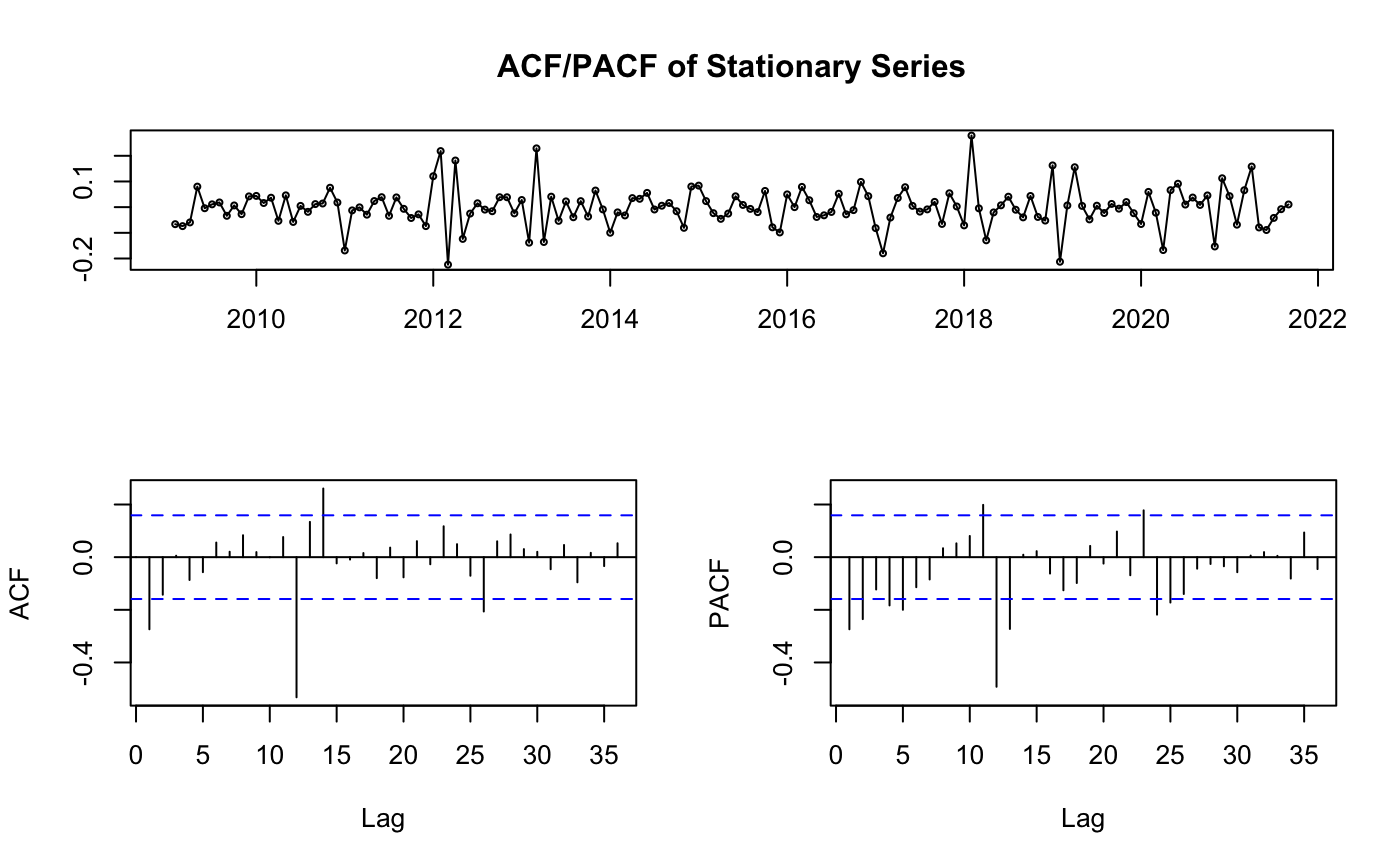
\includegraphics[width=1\linewidth]{images/ACF_PAC.png}
    \caption{ACF/PACF of Stationary Series}
    \label{fig:acf_pacf}
\end{figure}

By examining the ACF and PACF plots of a stationary series, Fig.\ref{fig:acf_pacf}, informed decisions can be made about which non-seasonal and seasonal AR and MA terms to include in a SARIMA model.\\

\begin{itemize}
\item \textbf{Seasonal order (P, Q)}:
    At lag 12 (the seasonal period), the ACF shows a significant negative spike, while the PACF stops at that lag. This behaviour is characteristic of a seasonal moving average component of order 1, suggesting that Q = 1 and P = 0.

\item \textbf{Non-seasonal order (p, q)}:
    At the non-seasonal lags, both the ACF and PACF exhibit significant spikes at lag 1. This ambiguity could indicate an autoregressive component of order 1 (p = 1), a moving average component of order 1 (q = 1), or potentially both.
\end{itemize}

Based on these observations, a reasonable candidate model is:
\[
\text{SARIMA}(p,1,q)(0,1,1)[12]
\]

However, the ACF and PACF plots are not entirely conclusive as they do not exhibit clear exponential decay or sharp cut-offs, which are typically used to identify pure AR or MA processes.

Due to this ambiguity, we opted to use the \textit{auto.arima()} function from the forecast package, which automates the model selection process by evaluating various combinations of (p, d, q)(P, D, Q) and selecting the model that minimises the AICc or BIC.

As this function handles logarithmic transformations and differencing internally when needed, we applied it directly to the original time series object \textit{ts\_data}.

\subsection{Automatic SARIMA Model Selection}

The function selected a \textbf{SARIMA(2,0,0)(0,1,2)[12]} model. This choice partially aligns with the expectations formed during the ACF and PACF analysis, where seasonal differencing and a seasonal MA component were anticipated. However, the selected non-seasonal AR order (p=2) was not fully evident in the initial visual analysis, highlighting the added value of automated methods in uncovering latent structure.\\

\begin{figure}[H]
    \centering
    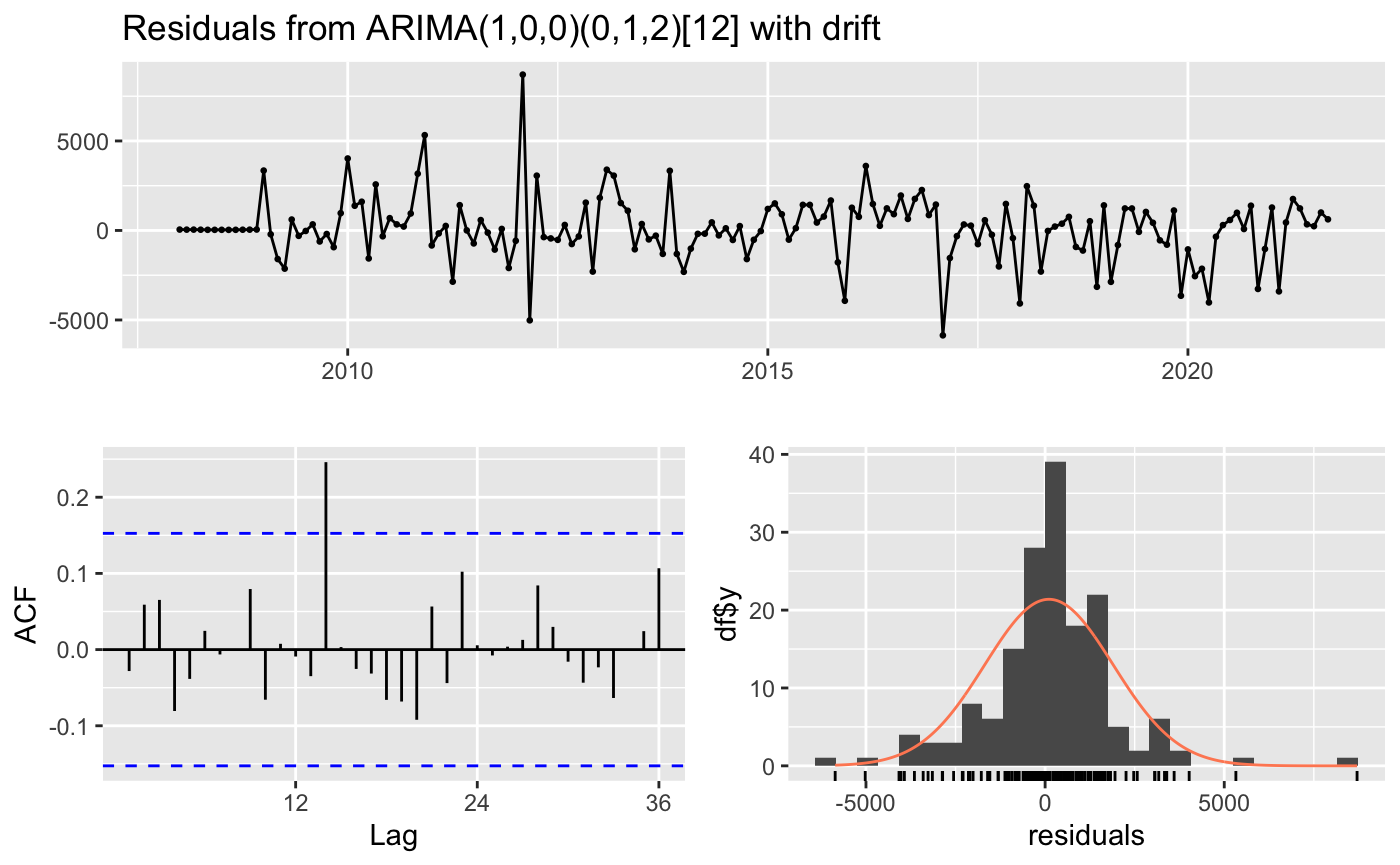
\includegraphics[width=1\linewidth]{images/residual_auto.png}
    \caption{Residuals Diagnostics ARIMA(1,0,0)(0,1,2)[12] (Auto.Arima)}
    \label{fig:residual_auto}
\end{figure}

\noindent\textbf{Residual Diagnostics}

To verify the adequacy of the fitted model, we performed diagnostic checks on the residuals, Fig.\ref{fig:residual_auto}. The diagnostic results showed the following:

\begin{itemize}
    \item The residuals plot reveals no discernible patterns and oscillates around a zero mean.
    \item The ACF of the residuals presents only one significant spike, suggesting minimal autocorrelation.
    \item The Ljung-Box test returns a high p-value (0.35), indicating no significant autocorrelation structure in the residuals.
\end{itemize}

These results confirm that the residuals behave like white noise, suggesting that the model captures the underlying structure of the training data effectively without patterns and non-autocorrelated.

\subsection{Manual SARIMA Model Specification}

As an alternative to automated model selection, we manually specified a SARIMA model based on analysis of the ACF and PACF plots of the stationary series. The chosen model \textbf{SARIMA(1,1,1)(0,1,1)[12]} reflects regular and seasonal differencing, both of which were deemed necessary from earlier transformation steps. We fitted the model to the training set using the \textit{arima()} function without including a drift term (as recommended when d = 1).

This alternative SARIMA model uses \( p = 1 \) and \( q = 1 \), values that were selected based on the non-seasonal lags of the ACF and PACF plots analyzed during the model identification phase.\\

\begin{itemize}
    \item \textbf{AR(1):} ar1=0.3651, significant (low standard error).
    \item \textbf{MA(1):} ma1=-0.9689, nearly -1, suggesting strong short-term smoothing.
    \item \textbf{Seasonal MA(1):} sma1=-1.0000, indicating strong seasonal dependence.
    \item \textbf{Standard error } = 0.1472, likely significant.
\end{itemize}

The estimated parameters are interpretable and appear to be statistically significant. When comparing information criteria to the previous automatic model \texttt{SARIMA(2,0,0)(0,1,2)[12]}, we observe that AIC, AICc, and BIC are lower, suggesting that the manual model achieves a better fit.\\

\noindent\textbf{Training Error Metrics}

\begin{itemize}
\item \textbf{ME:} -254.29 – small negative bias, suggesting slight underestimation.
\item \textbf{RMSE:} 1759.58 – relatively low magnitude of residual errors.
\item \textbf{MAPE:} 3.07\% – excellent accuracy (values below 10\% are typically acceptable).
\item \textbf{ACF1:} -0.028 – close to zero, indicating no residual autocorrelation.
\end{itemize}

\noindent\textbf{Residual Diagnostics}

We applied residual analysis to validate the adequacy of the model and the diagnostic plots show, Fig.\ref{fig:residual_manual}:

\begin{itemize}
    \item Residuals fluctuate randomly around zero with no visible structure.
    \item ACF of residuals shows one or two marginally significant spikes, but overall no meaningful autocorrelation.
    \item Ljung-Box test returns a p-value of 0.13, meaning we cannot reject the null hypothesis of independently distributed residuals.
\end{itemize}

\begin{figure}[H]
    \centering
    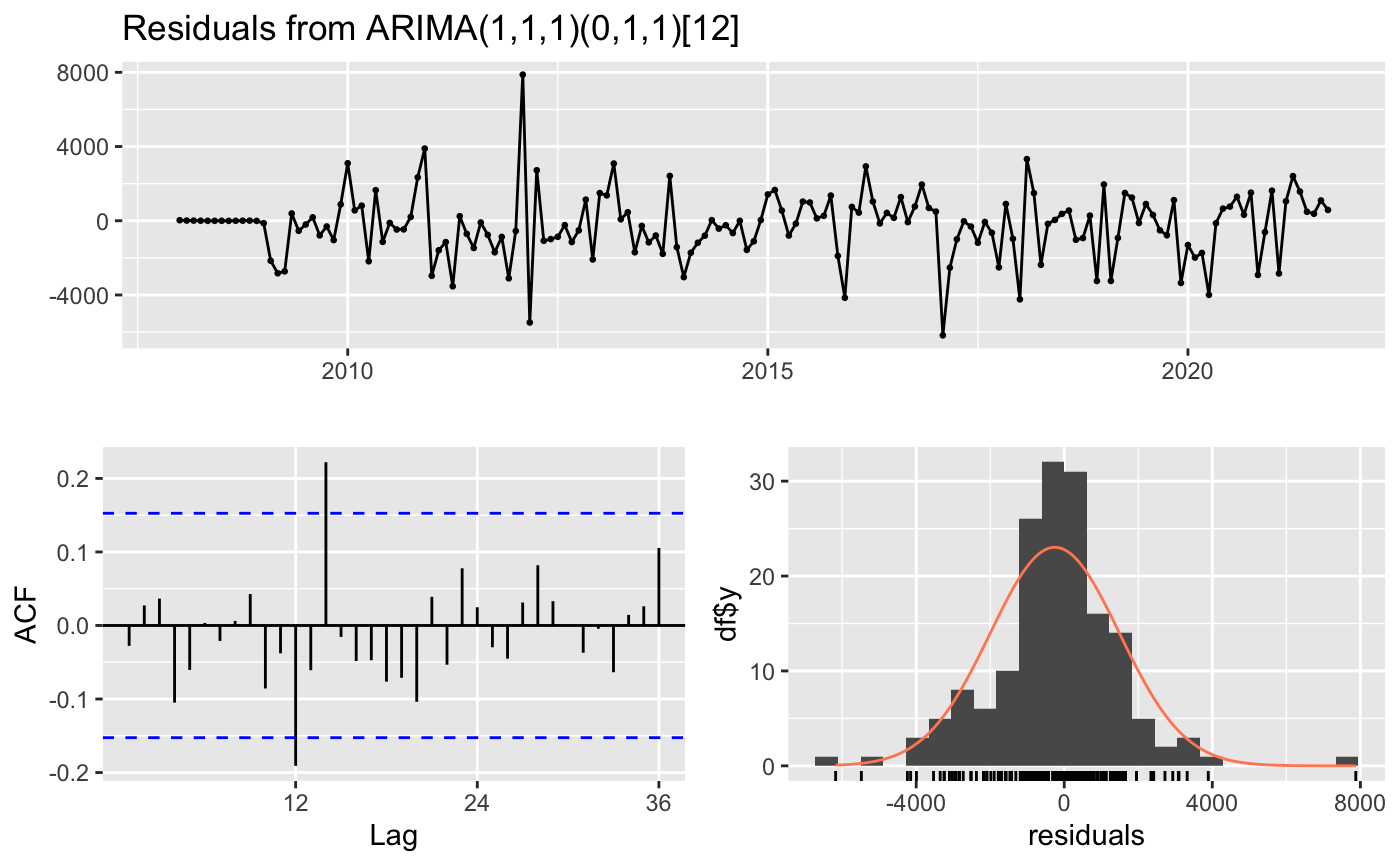
\includegraphics[width=1\linewidth]{images/manual_arima.png}
    \caption{Residuals Diagnostics SARIMA(1,1,1)(0,1,1)[12]}
    \label{fig:residual_manual}
\end{figure}


These results confirm that the model passes all diagnostic checks. The residuals behave like white noise, suggesting the model effectively captures the dynamics of the training series, similarly to the automatic SARIMA model.\\

\subsection{STL Decomposition Followed by ARIMA Modeling}

At this stage, we applied STL decomposition (seasonal-trend decomposition using loess), a technique that divides a time series into three components: trend, seasonality, and residuals. This makes it easier to model the residuals accurately, since the trend and seasonality have been removed. STL decomposition is particularly useful as it can be adjusted to be less sensitive to extreme values and more robust to outliers.\\

After decomposition, the residuals were modelled using an ARIMA model, which, in this case, fitted as an ARIMA(2, 1, 1). This strategy is effective in dealing with complexities or nonlinear variations in the seasonal components, enabling unstructured fluctuations to be modelled separately.\\

\begin{figure}[H]
    \centering
    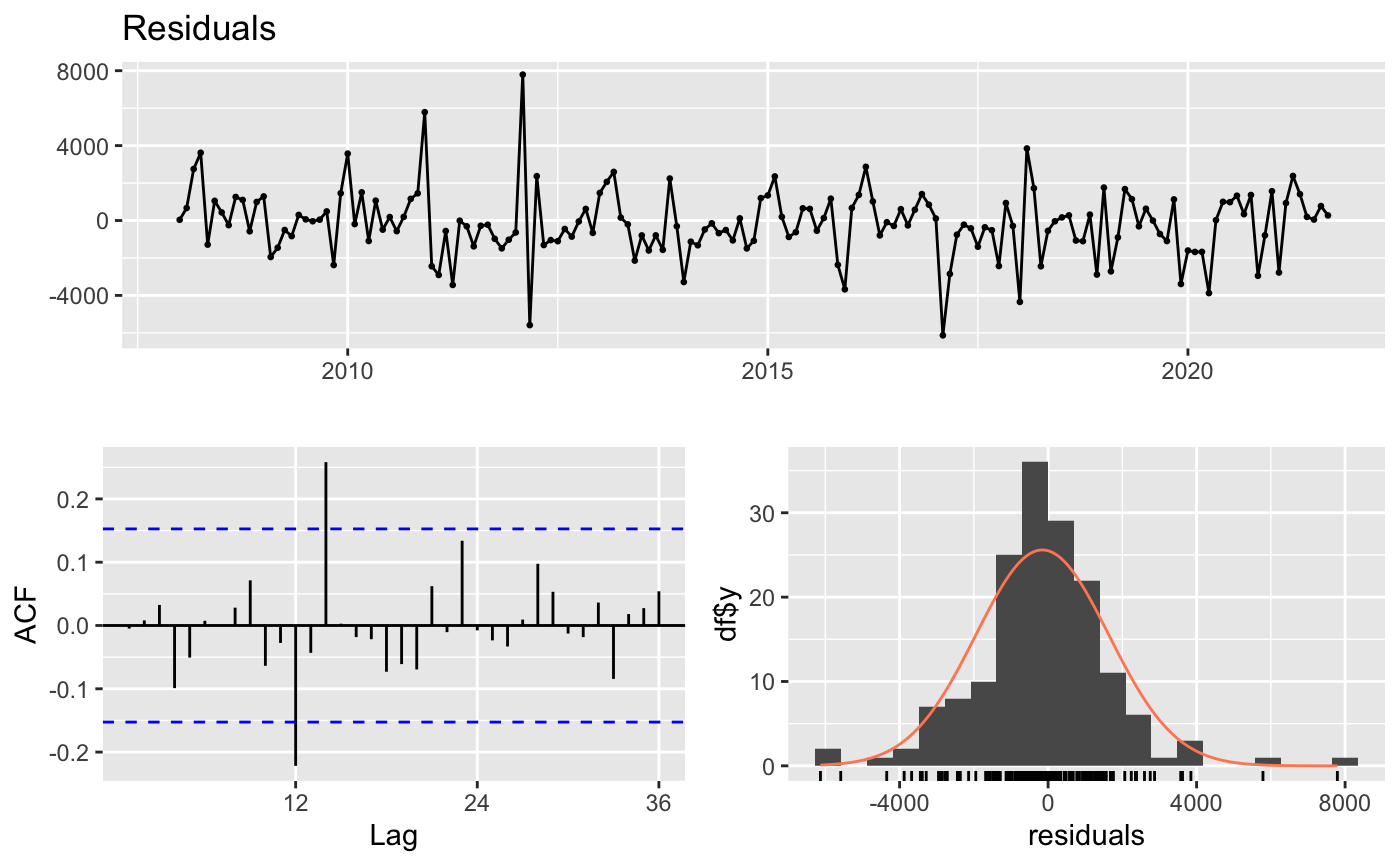
\includegraphics[width=1\linewidth]{images/st_red.png}
    \caption{Residuals Diagnostics STL decomposition with ARIMA(2,1,1)}
    \label{fig:st_red}
\end{figure}

 \noindent\textbf{Residual Diagnostics}

Analysis of the residuals from the STL + ARIMA model indicated that, Fig.\ref{fig:st_red}:
\begin{itemize}
    \item The residuals show no obvious patterns, oscillating randomly around zero.
    \item The autocorrelation function (ACF) of the residuals showed only a few isolated peaks, indicating that there is generally no significant correlation between the residuals.
    \item The Ljung–Box test showed a high p-value (0.11), implying that there is no evidence to reject the null hypothesis that the residuals are independent.
\end{itemize}

These results suggest that the model has successfully passed the diagnostic checks and that the residuals behave like white noise with no remaining systematic patterns or autocorrelation.

\subsection{Exponential Smoothing State Space Model (ETS)}

In this step, we fit an ETS model to the training data. The forecast package's \textit{ets()} function automatically selects the best model by testing various combinations of error, trend, and seasonality components (additive, multiplicative, and damped) and selecting the one with the lowest AICc value.

The ETS model is suitable for time series with systematic components, such as trends and seasonality, but with low noise. However, it does not address the issue of stationarity in the data, for which differentiation is recommended.

The selected model was ETS(M,Ad,M), which stands for:\\
- Error: Multiplicative (M)\\
- Trend: Additive Damped (Ad)\\
- Seasonality: Multiplicative (M)

This choice is consistent with the observed multiplicativity in the seasonality of the series, as well as incorporating a trend that amortises over time.\\

As for the smoothing parameters:\\
- Alpha (0.2592): a moderate value indicating a balance between the weight given to recent and past observations at series level.\\
- Gamma (1e-04) is practically zero, suggesting fixed seasonality over the period and low adaptability.

The seasonal vector shows variations over the 12-month cycle, with some months showing peaks, such as the winter months.

The sigma value (0.0445) indicates low residual variability, suggesting that the model reasonably well controls the residuals.\\

However, the information criteria (AIC and BIC) are considerably higher than those of previous models, suggesting that this model does not fit the series as well.
The residual autocorrelation (ACF1 approximatly 0.16) suggests that the residuals are slightly dependent. In addition, the model tends to underestimate the values, as indicated by the negative mean errors (ME and MPE).

This poorer fit can be explained by the non-stationarity of the data, which requires differentiation to stabilise the series, a transformation that the ETS model does not perform, thus compromising its fit.\\

\begin{figure}[H]
    \centering
    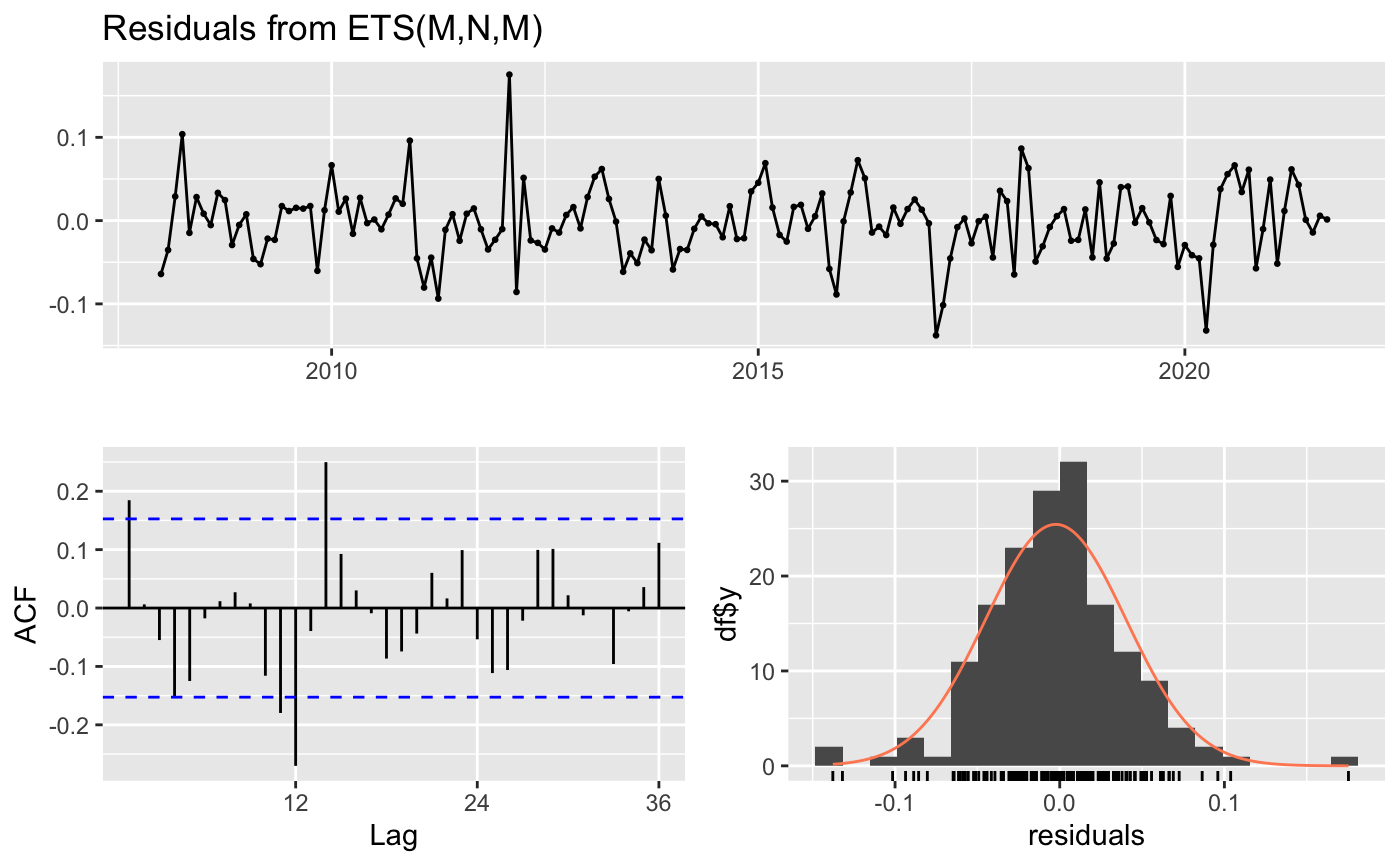
\includegraphics[width=1\linewidth]{images/ets_res.png}
    \caption{Residuals Diagnostics ETS(M,Ad,M)}
    \label{fig:res_ets}
\end{figure}

\noindent\textbf{Residual Diagnostics}

The graph of the residuals, Fig.\ref{fig:res_ets} shows random behaviour around zero, with no clear patterns.
The autocorrelation function of the residuals shows significant peaks, indicating residual correlation and the Ljung–Box test rejects the null hypothesis of residual independence, indicating that the residuals do not behave like white noise.

Therefore, the ETS model did not pass the diagnostic tests satisfactorily, as the residuals show significant autocorrelation, suggesting that patterns remain that the model has not captured.